\documentclass[]{article}
\usepackage{fullpage}
\usepackage{amsfonts}
\usepackage{amsmath}
\usepackage{graphicx}

\begin{document}

	\title{MAT 1320}
	\author{{\bf Calculus I}}
	\date{2013}
	\maketitle
	\begin{center}
		{\bf Prof:} Paul-Eug\`{e}ne Parent
	\end{center}
	\pagebreak
	\normalsize 
	\noindent{\bf Notations and symbols}\\

	\noindent Let $a\in\mathbb{R}$. We defined the \emph{absolute value} of $a$ by:
	$$
		 |a|:=\begin{cases}
			a\text{ if } a>0\\
			-a\text{ if }a<0
		\end{cases}
	$$
	\emph{Note: $:=$ is the "definition" sign.}\\
	The result is always a positive number.
	\begin{itemize}
		\item $|0|=0$
		\item $|3|=3$
		\item $|-2|=2$
		\item $|\sqrt{2}-1|=\sqrt{2}-1$
	\end{itemize}
	{\bf Properties of the absolute value}
	\begin{itemize}
		\item $|ab|=|a||b|$
		\item if $b\ne 0$, then $|\frac{a}{b}|=\frac{|a|}{|b|}$
	\end{itemize}
	If $a>0$, then
	\begin{itemize}
		\item Solve $|2x-5|=3$
		\item {\bf Solution:} We have two cases to consider:\\
		$2x-5=3$, which leads to $x=4$,\\
		$-(2x-5)=3$, which leads to $x=1$\\
		Hence the result: $x=1$ or $4$
		\item Solve $|3x+2|\ge 4$\\
		Either $3x-2>4$, which leads to $x\ge\frac{2}{3}$\\
		Or $3x+2\le -4$, which leads to $x\le -2$\\
		Hence the result $x\in ~]-\infty,-2]\cup[\frac{2}{3},+\infty [$
	\end{itemize}
	{\bf Small remarks on the square root function:}\\
	By definition, its \emph{domain}, i.e. the allowed numbers that can feed into the quare root, is
	$$x\in~[0, +\infty[$$
	While its \emph{range}, i.e. what values the square root can "spit out", is
	$$y\in~[0,+\infty[$$
	We usually encompass all this information in a neat, compact form, i.e.:
	$$\sqrt{\cdot}:~[0,+\infty[~\rightarrow~[0,+\infty[$$
	$$x\mapsto\sqrt{x}$$
	Where the second line gives the actual transformation recipe.
	\pagebreak\\
	We can extend this to all functions, i.e.
	$$f:D\longrightarrow R$$
	$$x\mapsto f(x)$$
	Where we recover at once on the first line the name of the function $f$, its domain $D$, and its range $R$, while the second line gives us the explicit transformation rule.\\
	Ex:
	$$g:\mathbb{R}\longrightarrow\mathbb{R}$$
	$$x\mapsto x^3\cdot\sin(x)=g(x)$$
	That being said, what is:
	$$\sqrt{a^2}=|a|$$
	The range of a square root function is always $[0,+\infty[$. Indeed... $\sqrt{(-3)^2}=\sqrt{9}=3=|-3|$\\
	The square root function \emph{is a one-to-one function}.\\
	$$|a|=\sqrt{a^2}$$
	\pagebreak\\
	{\bf Recall}\\
	We will denote a function $f$ by
	$$f:D\rightarrow R$$
	$$x\mapsto f(x)$$
	Where $D$ is the domain of $f$, $R$ is its range, and $f(x)$ is the actual transform rule.\\\\
	{\bf Definition}\\
	The \emph{image} of $f$, denoted $f(D)$, is the set of all $y\in R$ such that there exists at least one $d\in D$ with
	$$f(d)=y$$
	\underline{Example:} Consider the squaring function:
	$$(\cdot)^2:\mathbb{R}\rightarrow\mathbb{R}$$
	$$x\mapsto  x^2$$
	This leads to\\
	{\bf Definition}\\
	A function is onto (ur surjective) if its image is equal to its range.\\
	\underline{Examples}:
	\begin{itemize}
		\item $x^2$ is not onto
		\item $x^3$ is onto
	\end{itemize}
	\begin{center}
		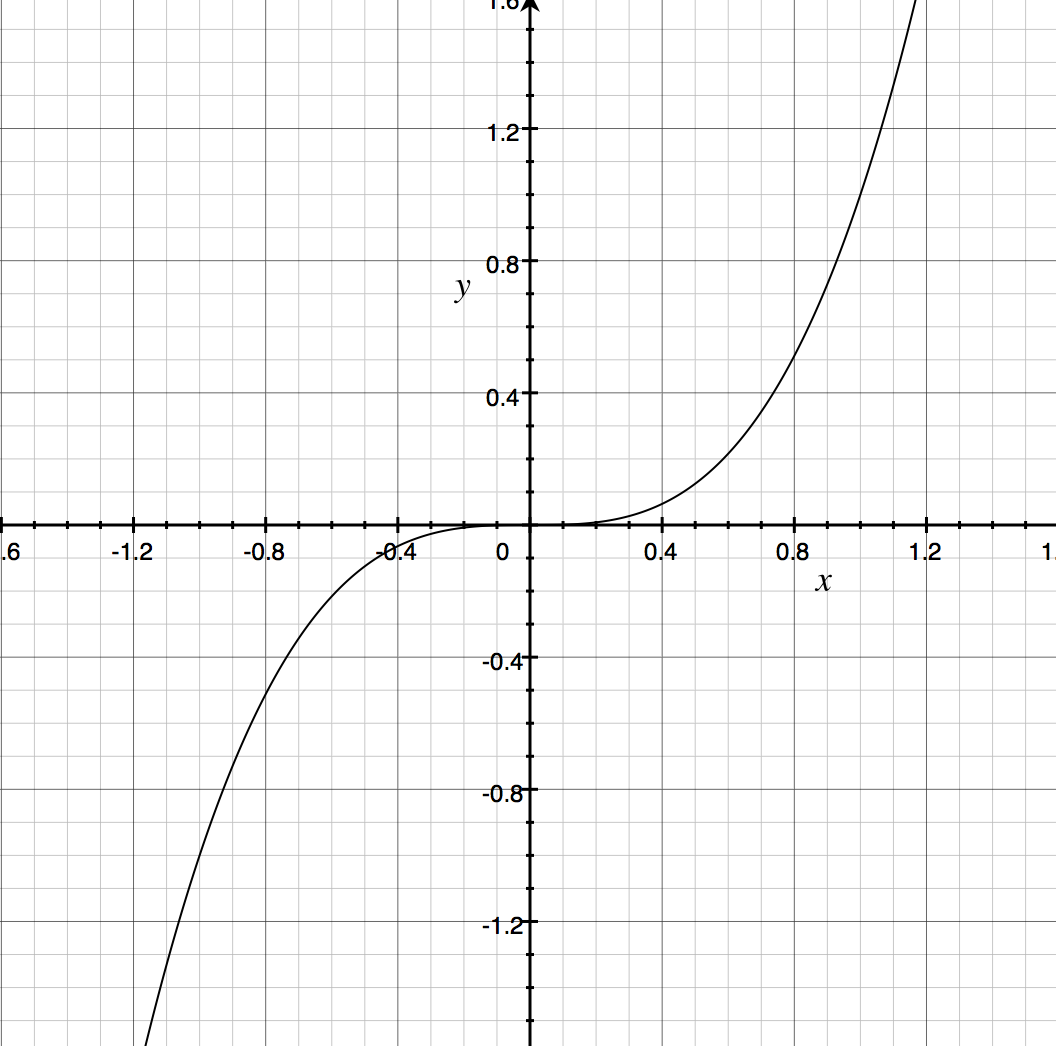
\includegraphics[scale=0.4]{./graphics/x3.png}\\
		\emph{The function, $x^3$}\\
	\end{center}
	{\bf Definition}\\
	A function is \emph{one-to-one} or \emph{injective} if whenever $f(x_1)=f(x_2)$, we then must have $x_1=x_2$.\\
	In other words, a one-to-one function cannot produce more than once a given value.\\
	\underline{Examples:}\\
	\begin{itemize}
		\item The squaring function is {\bf not} one-to-one because\\
		$(-2)^2=2^2$ but $-2\ne 2$
		\item The cubic function is one-to-one.
	\end{itemize}
	If a function $f$ is both onto \emph{and} one-to-one, it's called a \emph{bijection}.\\
	{\bf Theorem}\\
	A function $f:A\longrightarrow B$ is a bijection if and only if there exists a function $f^{-1}:B\longrightarrow A$ such that:
	\begin{itemize}
		\item $f^{-1}(f(a))=a$ for all $a\in A$, and
		\item $f(f^{-1}(b))=b$ for all $b\in B$
	\end{itemize}
	{\bf Remarks:}\\
	\begin{itemize}
		\item If such  a function exists, then it is unique. It is called the inverse of $f$.
		\item We must have
		$$b=`f(a) \iff a=f^{-1}(b)$$
		\item\underline{\bf WARNING:}
		$$f^{-1}(x)\ne\frac{1}{f(x)}$$
		$$(f(x))^{-1}=\frac{1}{f(x)}$$
	\end{itemize}
	\underline{Example}\\
	Find the inverse of $f(x)=x^3+2$.\\
	\underline{Solution}
	\begin{itemize}
		\item Write $y=x^3+2$
		\item Solve for $x$ as a function of $y$, i.e.
		\begin{itemize}
			\item $x^3=y-2$ hence $x=(y-2)^{1/3}$
		\end{itemize}
		\item Switch $x$ and $y$, i.e. $y=(x-2)^{1/3}$
	\end{itemize}
	Checking computations with...
	\begin{itemize}
		\item$f(f^{-1}(x))=f((x-2)^{1/3})\\
		=((x-2)^{1/3})^3+2\\
		=x-2+2=x$
	\end{itemize}
	The function $\sqrt{x}$ is not the inverse of $x^2$.\\
	Recall that $\sqrt{x^2}=|x|$ and not $x$ is neither one-to-one nor onto, and hence is not invertible!\\\\
	But we can consider a new function with a smaller domain and a smaller range but with the same transformation rule.
	$$h:~[0,+\infty[~\longrightarrow~[0,+\infty[$$
	$$x\mapsto x^2$$
	Now that function is a bijection and its inverse is $\sqrt{x}$, i.e. $\sqrt{h}=x$ and $(\sqrt{x})=x$
	\pagebreak\\
	\Large{Logarithms}\\
	\normalsize{\bf Remarks:}\\
	1. $f_a$ is hence one-to-one, and\\
	2. If we restrict the range of $f_a$ to $]0,+\infty[$, then$f_a$ becomes a bijection.\\
	We denote ints inverse by
	$$\log_a(x)$$
	The number $a$ is called the base\\
	If the base is omitted as in $\log 5$, it is assumed to be base 10\\
	When $a=e\approx 2.71828$, the log is written
	$$\ln(x)$$
	Recall that for $1\ne a>0$ we have the exponential function:
	$$f_a:\mathbb{R}\longrightarrow\mathbb{R}$$
	$$x\mapsto a^x$$
	which is 
	\begin{itemize}
		\item strictly decreasing if $a>1$; and
		\item strictly increasing if $a<1$.
	\end{itemize}
	\underline{Remarks}:\\
	1. $f_a$ is hence one-to-one, and\\
	2. $f_a(x)>0$.\\
	Hence if we restrict the range of $f_a$ to $]0,+\infty[$, then $f_a$ becomes a bijection.\\
	We denote its inverse by $log_a(x)$\\
	This function is characterized by:
	$$
	log_a(x)=y\iff a^y=x
	$$
	\begin{itemize}
		\item The number $a$ is called the \emph{base}
		\item If the base is omitted as in $log(5)$, it is assumed to be 10.
		\item When $a=e\approx 2.71828$, we write $\ln(x)$, and we call it the natural logarithm.
	\end{itemize}
	\begin{center}
		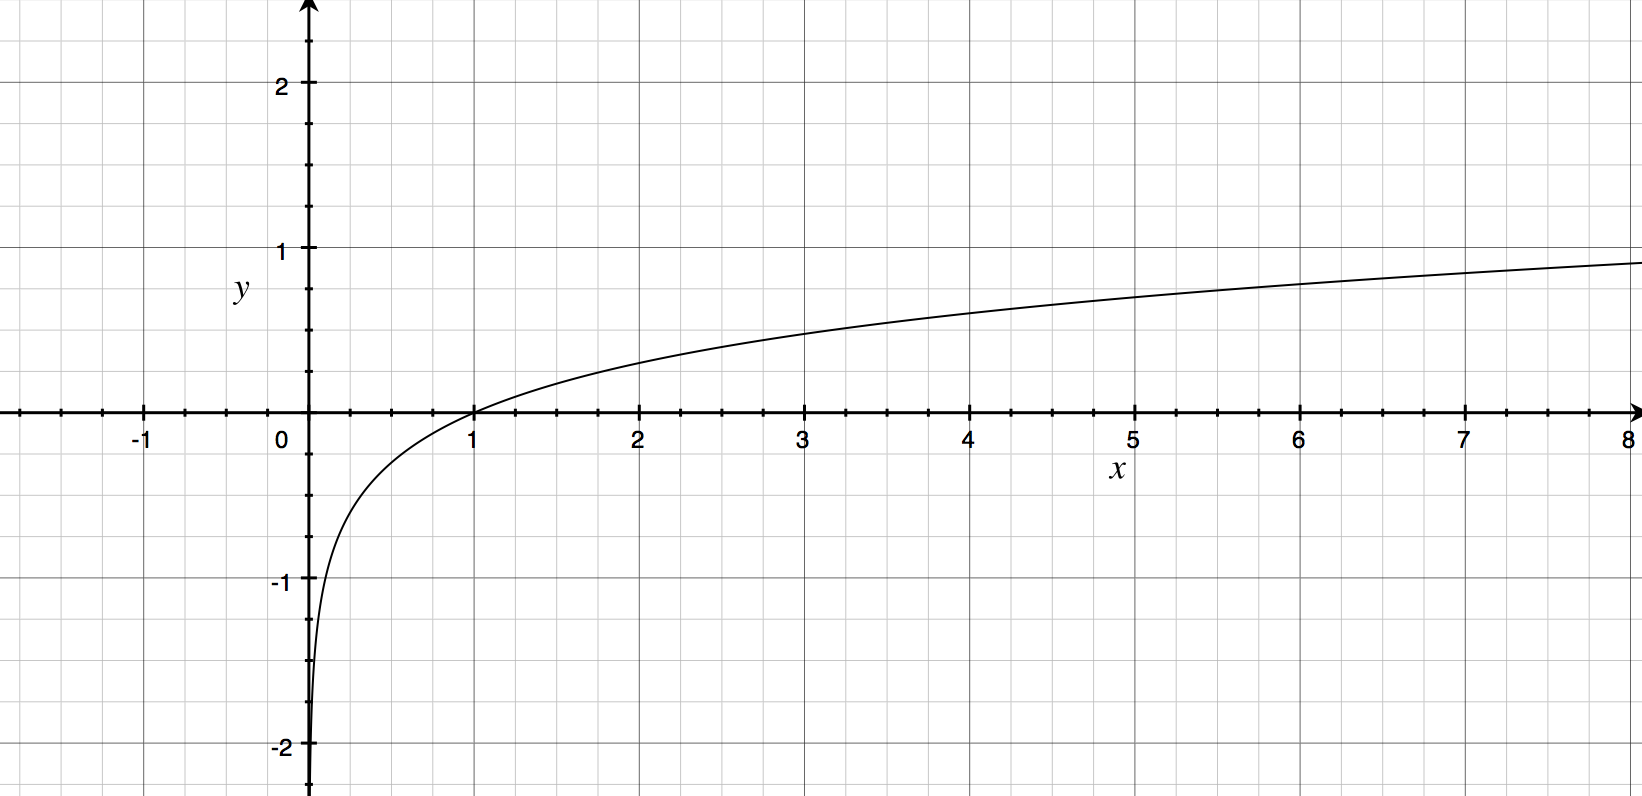
\includegraphics[scale=0.4]{./graphics/logx.png}\\
		\emph{$\log(x)$}
	\end{center}
	Compute $\log_2(80)-\log_2(5)$
	\begin{align*}
		\log_2(80)-\log_2(5)&=\log_2\frac{80}{5}\\
		&=\log_2(16)\\
		&=4
	\end{align*}
	Theorem:\\
	Let $1\ne a>0$ and $x>0$. Then:
	$$\log_a(x)=\frac{\ln(x)}{\ln(a)}.$$
	Why is this true?\\
	If $y=\log_a(x)$, then $a^y=x$. Applying $\ln$ to both sides we get:
	$$
	\ln(x)=\ln(a^y)=y\ln a.
	$$
	Hence $y=\frac{\ln(x)}{\ln(a)}$.\\\\
	Compute with a precision of six decimal places
	$$
	\log_8(5).
	$$
	\underline{Solution:} $\log_8(5)=\frac{\ln(5)}{\ln(8)}\approx 0.773976$\\\\
	Solve $e^{5-3x}=10$\\
	\underline{Solution:}\\
	Apply $\ln$ to both sides\\
	Solve for $x$, i.e. $x=\frac{5-\ln(10)}{3}\approx 0.899138$\\\\
	\pagebreak\\
	\Large{Trigonometry}\\
	\large{Inverse trig functions}\\
	\normalsize
	Consider a circle of radius $r$ and some arc of length $a$ and $c$ its circumference.\\
	On a unit circle,
	\begin{itemize}
		\item A(0)=(1,0) implies $\cos(0)=1$ and $\sin(0)=0$
	\end{itemize}
	{\bf Properties}\
	The function $A(\theta)$ is periodic of a period of $2\pi$, i.e. $A(\theta)=A(\theta+2\pi)$. Hence:
	$$
	\cos(\theta)=\cos(\theta+2\pi)\text{ and }\cos(\theta)=\cos{\theta-2\pi}
	$$
	As one can deduce by either their respective definitions or their associated graphs,
	\begin{itemize}
		\item The function $\sin\theta$ is an odd function
		\item The function $\cos\theta$ is an even function
	\end{itemize}
	\begin{center}
		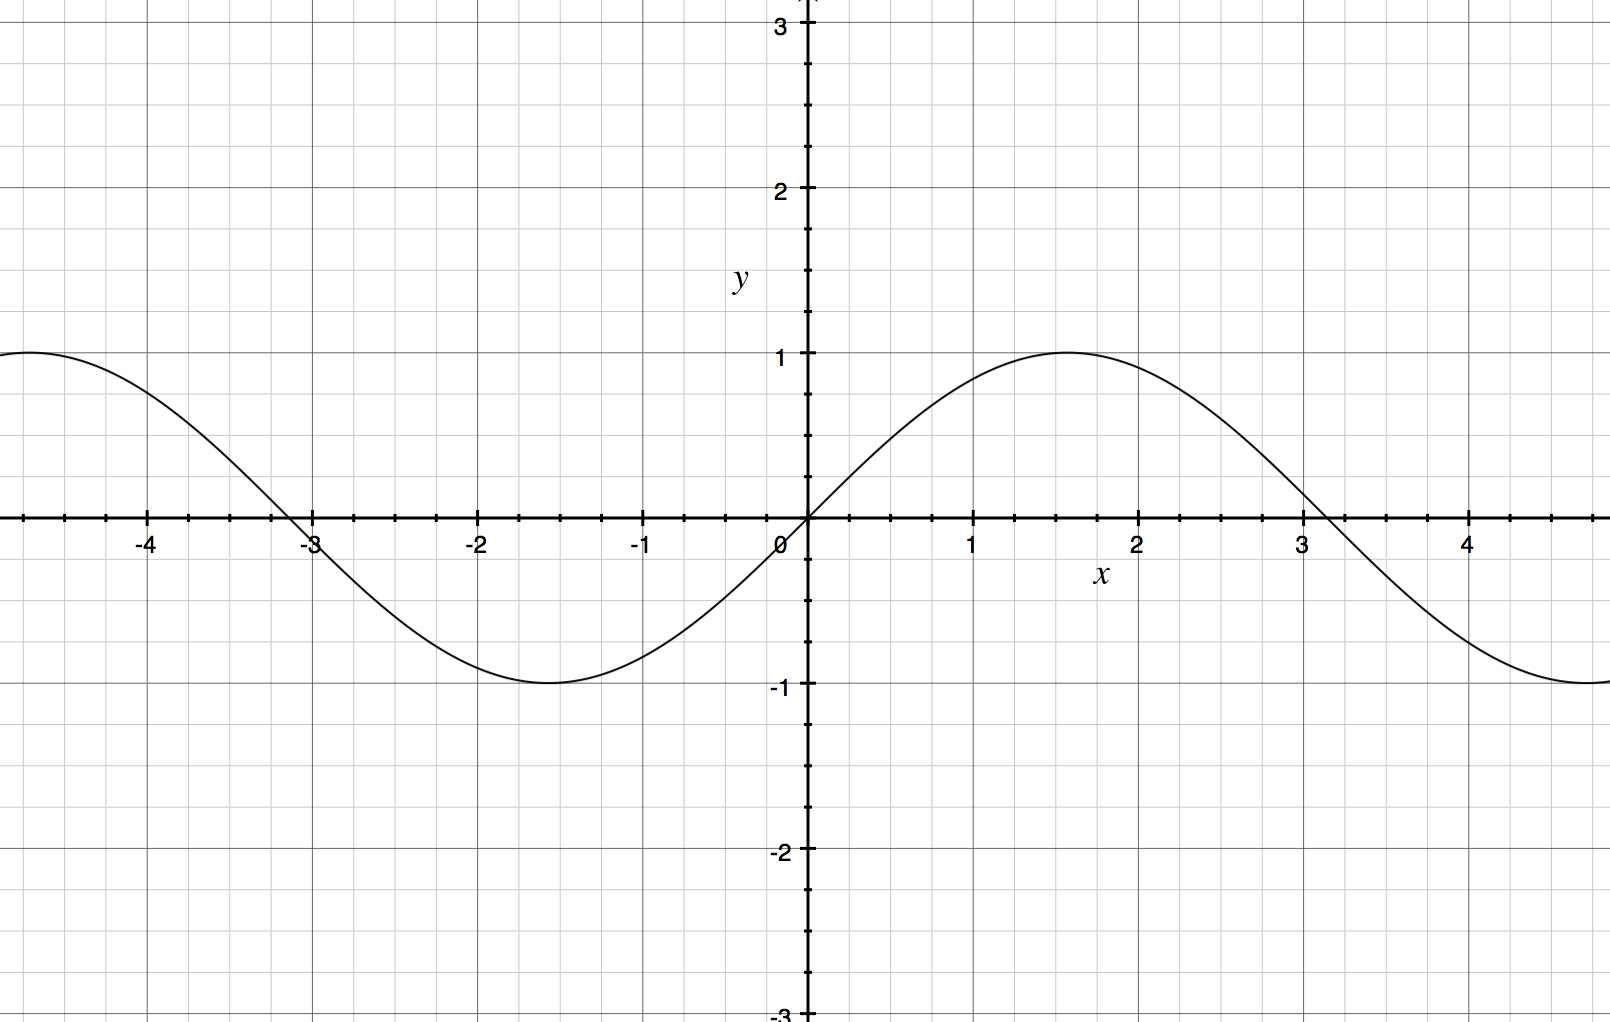
\includegraphics[scale=0.4]{./graphics/sinx.png}\\
		$\sin(x)$
	\end{center}
	{\bf Other trig functions}
	$$
	\tan(\theta):=\frac{\sin(\theta)}{\cos{\theta}}\text{ and }\cot{\theta}=\frac{\cos(\theta)}{\sin(\theta)}
	$$
	\begin{center}
		Secant and cosec
	\end{center}
	From $\cos^2(\theta)+\sin^2(\theta)=1$ one can define:\\
	$1+\tan^2(\theta)=\sec^2(\theta)$\\\\
	{\bf To do at home: }
	Show that:\\
	\begin{itemize}
		\item $\sin(2x)=2\sin(x)\cos(x)$
		\item
			\begin{align*}
				\cos(2x)&=\cos^2(x)-\sin^2(x)\\
				&=2\cos^2(x)-1\\
				&=1-2\sin^2(x)
			\end{align*}
	\end{itemize}
	\pagebreak
	Find all $x\in[0,2\pi]$ such that $\sin(x)=\sin(2x)$\\
	\underline{Solution:} Recall that $\sin(2x)=2\sin(x)\cos(x)$, hence we need to solve\\
	$\sin(x)=2\sin(x)\cos(x)$. Equivalently, $\sin(x)(1-2\cos(x))=0$.\\
	We have two cases:
	\begin{itemize}
		\item $\sin(x)=0$, which implies that $x=0, \pi, or 2\pi$, or
		\item $1-2\cos(x)=0$, which implies $\cos(x)=\frac{1}{2}$, or equivalently $x=\frac{\pi}{3}$ or $\frac{5\pi}{3}$
	\end{itemize}
	Conclusion: The solutions are $x=0,\frac{\pi}{3},\pi,\frac{5\pi}{3},$ or $2\pi$\\\\
	We want to "invert" the trigonometric functions. Recall that the domain and the range of $\sin(x)$ and $\cos(x)$ are the real numbers. Two problems arise:
	\begin{itemize}
		\item both functions are periodic, hence they are not one-to-one
		\item both functions are not onto as their images are $[-1,1]$
	\end{itemize}
	We then need to consider \emph{restricted} versions of those functions if we want to proceed.\\
	In the case of $y=\sin(x)$, we consider the classical domain 
	$$[-\frac{\pi}{2},\frac{\pi}{2}]\longrightarrow[-1,1]$$
	$$x\mapsto\sin(x)$$
	Hence the function $y=Sin(x)$ is now onto and one-to-one and thus admits and inverse function
	$$
	\arcsin~:~[-1,1]\longrightarrow[-\frac{\pi}{2},\frac{\pi}{2}].
	$$
	In particular,\\
	\begin{itemize}
		\item $\arcsin(Sin(x))=x~\forall~x\in[-\frac{\pi}{2},\frac{\pi}{2}]$
		\item $Sin(\arcsin(x))=x~\forall~x\in[\frac{-1}{1}]$
		\item $y=\arcsin(x)\iff Sin(y)=x$
	\end{itemize}
	\begin{center}
		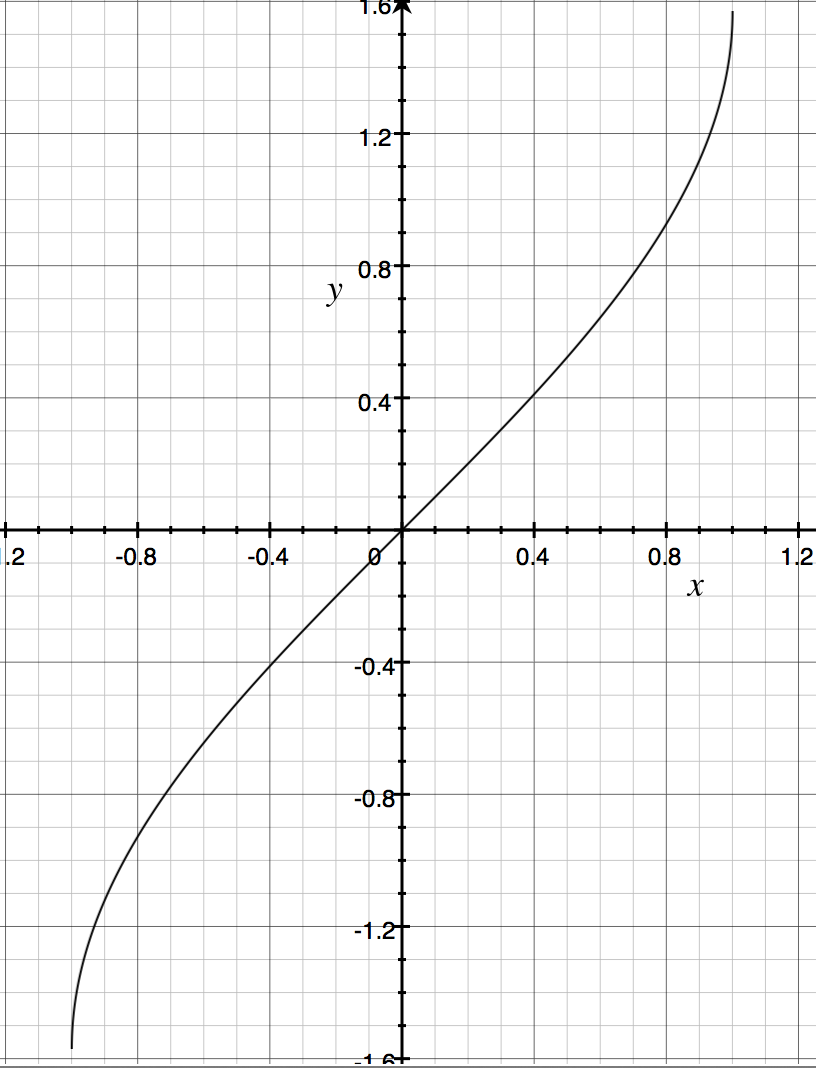
\includegraphics[scale=0.4]{./graphics/arctanx.png}\\
		$\arctan(x)$
	\end{center}
	NOTE: trig functions with caps first letter are informal notation to denote processed sine and cosine functions
	\pagebreak\\
	{\bf Exercises}\\
	Simplify the expression $\cos(\arctan(x))$\\
	\underline{Solution}:
	$$y=\arctan(x)\iff Tan(y)=x \text{ for } y\in~]-\frac{\pi}{2},\frac{\pi}{2}[$$
	On the other hand, we have the trigonometric identity:
	\begin{align*}
		\sec^2(x)&=1+\tan^2(y)\\
		&=1+x^2\text{ why?}
	\end{align*}
	Finally,
	$$
	\cos(\arctan(x))=\cos(y)=\frac{1}{\sec(y)}=\frac{1}{\sqrt{1+x^2}}\text{ ... why?}
	$$
	Compute exactly $\tan(\arcsin(1/3))$\\
	\underline{Solution}\\
	$$
		\theta=\arcsin(1/3)\iff Sin(\theta)=1/3\text{ when }\theta\in~[-\frac{\pi}{2},\frac{\pi}{2}],
	$$
	On the other hand, we  have the trigonometric identity $\cos^2\theta=1-\sin^2\theta$
	\pagebreak\\
	\Large{Limits}\\
	\normalsize
	Let $f:D\rightarrow\mathbb{R}$ be a function, $L\in\mathbb{R}$ and $a\in\mathbb{R}$ a point of either $D$ or a boundary point of $D$.\\
	\underline{Examples of acceptable $a$:}
	\begin{itemize}
		\item If $D=[1,2]$, then $a$ could be 1.5
		\item If $D=]1,3[$ then $a$ could also be 3 or -1, even though they are not in the domain of $f$.
	\end{itemize}
	{\bf Definition:}\\
	We will write:
	$$
		\lim_{x\to a}f:D
	$$
	\underline{Remark:} That value $L$ must be independent of the way we approach $a$.\\\\
	We can expand the definition of limits and ask, "is $f(x)$ approaching a definite value as $|x|$ grows arbitrarily?" We write in this case either:
	$$
		\lim_{x\to \infty}f(x)~~~\text{or}~~~\lim_{x\to-\infty}f(x)
	$$
	In the case of $y=\frac{1}{x}$ we have:
	$$
		\lim_{x\to\infty}f(x)=\lim_{x\to -\infty}f(x)=0
	$$
	{\bf Directional limits}\\
	In some problems, we might be interested in only a certain direction of approach.\\
	If we approach $a$ from the right, we write:
	$$
		\lim_{x\to a^+}f(x)
	$$
	Conversely, if we approach $a$ from the left, we write:
	$$
		\lim_{x\to a^-}f(x)
	$$
	{\bf Theorem:}\\
	The limit $\lim\limits_{x\to a}f(x)$ exists iff both the right and left limit exist and are equal.\\
	
	\noindent Suppose both $\lim\limits_{x\to a}f(x)$ and $\lim\limits{x\to a}g(x)$ are numbers and let $c\in\mathbb{R}$.
	\begin{itemize}
		\item $\lim\limits_{x\to a}(f(x)\pm g(x))=\lim\limits_{x\to a}f(x)\pm\lim\limits_{x\to a}g(x)$
		\item $c\lim\limits_{x\to a}f(x)=\lim\limits_{x\to a}c(f(x))$
		\item $\lim\limits_{x\to a}f(x)g(x)=\left( \lim\limits_{x\to a}f(x) \right)\left( \lim\limits_{x\to a}g(x) \right)$
		\item $\lim\limits_{x\to a}\frac{f(x)}{g(x)}=\frac{\lim\limits_{x\to a}f(x)}{\lim\limits_{x\to a}g(x)}\text{ if }\lim\limits_{x\to a}g(x)\ne 0$
	\end{itemize}
	{\bf Definition}
	Let $f:D\rightarrow\mathbb{R}$ be a function and $a\in D$. We say that $f$ is \emph{continuous at} $a$ if:
	$$
		f(a)=\lim_{x\to a}f(x)
	$$
	{\bf Examples of continuous functions}
	\begin{itemize}
		\item All polynomial functions
		\item All trig functions
		\item All exponential and log functions
		\item All rational functions
	\end{itemize}
	\underline{\bf Warning:} One checks continuity only on $x$ belonging to the domain of a function.\\
	\underline{Question:} Is $\frac{1}{x}$ continuous? Yes, since it is not defined on $x=0$\\\\
	Compute:
	$$
		\lim_{x\to 0}\frac{(3+x)^2-9}{x}
	$$
	Solution: First of all we notice that it is a rational function but 0 is not in its domain. Hence we can't simply substitute 0 in the expression. Thus:
	\begin{align*}
		\lim_{x\to 0}\frac{(3+x)^2-9}{x}&=\lim_{x\to 0}\frac{9+6x+x^2-9}{x}\\
		&=\lim_{x\to 0}\frac{x(6+x)}{x}
	\end{align*}
	As we are interested in the limit when approaching 0, we are purposely avoiding $x=0$, hence:
	$$
		\lim_{x\to 0}\frac{(3+x)^2-9}{x}=\lim_{x\to 0}(6+x)
	$$
	And now we notice that the function $6+x$ is a line (hence continuous) and that 0 is in its domain.\\
	\underline{Conclusion}: $\lim\limits_{x\to 0}\frac{(3+x)^2-9}{x}=\lim\limits_{x\to 0}(6+x)=6+0=6$\\
	Let $f,~g:D\rightarrow\mathbb{R}$ be two continuous functions (when we do not specify at a particular point we mean continuous everywhere on their domain).
	\begin{itemize}
		\item $f\pm g$ is continuous;
		\item $f\cdot g$ is continuous, and
		\item $\frac{f}{g}$ is continuous whenever the quotient is defined, i.e. it is continuous on all $x\in D$ such that $g(x)\ne 0$.	
	\end{itemize}
	Let $f:D\rightarrow\mathbb{R}$ be a continuous function and suppose that there is an interval $[a,b]\subseteq D$\\
 	{\bf Theorem}\\
	For each $y$ between $f(a)$ and $f(b)$, there is $x_0\in[a,b]$ such that $y=f(x_0)$\\
	Suppose that we have a continuous function $f:[0,1]\rightarrow[0,1]$\\
	Then one knows that there is $x_0\in[0,1]$ such that $f(x_0)=x_0$, i.e. $f$ admits a fixed point.\\
	Why?\\
	Consider the new function
	\begin{align*}
		g:[0,1]&\longrightarrow\mathbb{R}\\
		x&\mapsto f(x)-x
	\end{align*}
	On one hand, if $f(1)=1$, then we are done as we have found a fixed point. Else by construction
	$$
		g(1)<0\text{ since }f(1)<1
	$$
	On the other hand, if $f(0)=0$ then again we are done. Else by construction
	$$
		g(0)>0\text{ since }f(0)>0
	$$
	\pagebreak\\
	{\bf General culture}\\
	This result is true in higher dimensions!\\
	It is known as the \emph{Brouwer fixed-point theorem}.\\
	{\bf Theorem:}\\
	Let $f:[0,1]^n\rightarrow[0,1]^n$ be a continuous function for $n=1,2,3,...$. There exists $x_0\in[0,1]^n$ such that:
	$$
		f(x_0)=x_0
	$$\\
	{\bf Second hypothesis}\\
	Let $p(x)=x^n+a_{n-1}x^{n-1}+...+a_1x+a_0$ be a polynomial of odd degree grate or equal to 1, i.e. $n$ can only be an odd positive integer greater than or equal to one.\\
	{\bf Theorem}\\
	One automatically knows that there is at least one $x_0\in\mathbb{R}$ such that
	$$
		p(x_0)=0
	$$
	Why?\\
	Intuitively, we know that
	$$
		\lim_{x\to\pm\infty}p(x)=\lim_{x\to\pm\infty}x^n
	$$
	Moreover, on one hand:
	$$
		\lim_{x\to\infty}x^n=\infty
	$$
	i.e. there is a $b\in\mathbb{R}$ such that $p(b)>0$.\\
	On the other hand, we also know that since $n$ is odd,
	$$
		\lim_{x\to-\infty}x^n=-\infty
	$$
	i.e. there is $a\in\mathbb{R}$ such that $p(a)<0$\\
	Conclusion: By the intermediate value theorem there must exist $x_0\in[a,b]$ such that:
	$$
		p(x_0)=0
	$$\\
	\pagebreak\\
	\Large{The derivative}\\
	\normalsize
	{\bf Outline}
	\begin{enumerate}
		\item Geometric interpretation
		\item The derivative as a function
		\item Computation\\
	\end{enumerate}
	{\bf Recall:}\\
	Let $f:D\rightarrow\mathbb{R}$ be a function and $x_0\in D$.\\\\
	{\bf Definition:}\\
	We say that $f$ is differentiable at $x_0\in D$ if the following limit:
	$$
		\lim_{h\to 0}\frac{f(h+x_0)-f(x_0)}{h}
	$$
	is a number, i.e. it exists.\\
	In that case we denote the number $f'(x_0)$.\\
	The question is, what does it mean to differentiate a function at $x_0$?\\
	Recall how one computes the slope of a line:
	$$
		m=\frac{\Delta y}{\Delta x}
	$$
	Hence in the case of the line $\mathbb{D}$, we have
	$$
		m_{\mathbb{D}}=\frac{f(x_0+\Delta x)-f(x_0)}{\Delta x}
	$$
	Now as $\Delta x$ goes towards 0, the slope $m_D$ goes towards the slope of the red line.\\\\
	{\bf Continuity?}\\
	Suppose $f:D\rightarrow\mathbb{R}$ is differentiable at $x_0\in\mathbb{R}$.\\
	Pick and $x\in D$ but such that $x\ne x_0$. Then
	\begin{align*}
		f(x)&=f(x)+0\\
		&=f(x)-f(x_0)+f(x_0)\\
		&=(f(x)-f(x_0))\cdot 1+f(x_0)\\
		&=(f(x)-f(x_0))\frac{x-x_0}{x-x_0}+f(x_0)\\
		&=\frac{f(x)-f(x_0)}{x-x_0}(x-x_0)+f(x_0)
	\end{align*}
	And now we can take the limit on each side, i.e.
	\begin{align*}
		\lim_{x\to x_0}&=\lim_{x\to x_0}\left(\frac{f(x)-f(x_0)}{x-x_0}(x-x_0)+f(x_0)\right)\\
		&=\left(\lim_{x\to x_0}\frac{f(x)-f(x_0)}{x-x_0}\lim_{x\to x_0}(x_{x_0})+\lim_{x\to x_0}f(x_0)\right)\\
		&=f'(x_0)\cdot 0+f(x_0)\\
		&=f(x_0)
	\end{align*}
	{\bf Conclusion:} $f$ is continuous at $x_0$.\\
	\underline{Warning:} The converse is false, i.e. a continuous function is not necessarily differentiable.\\
	\begin{center}	
		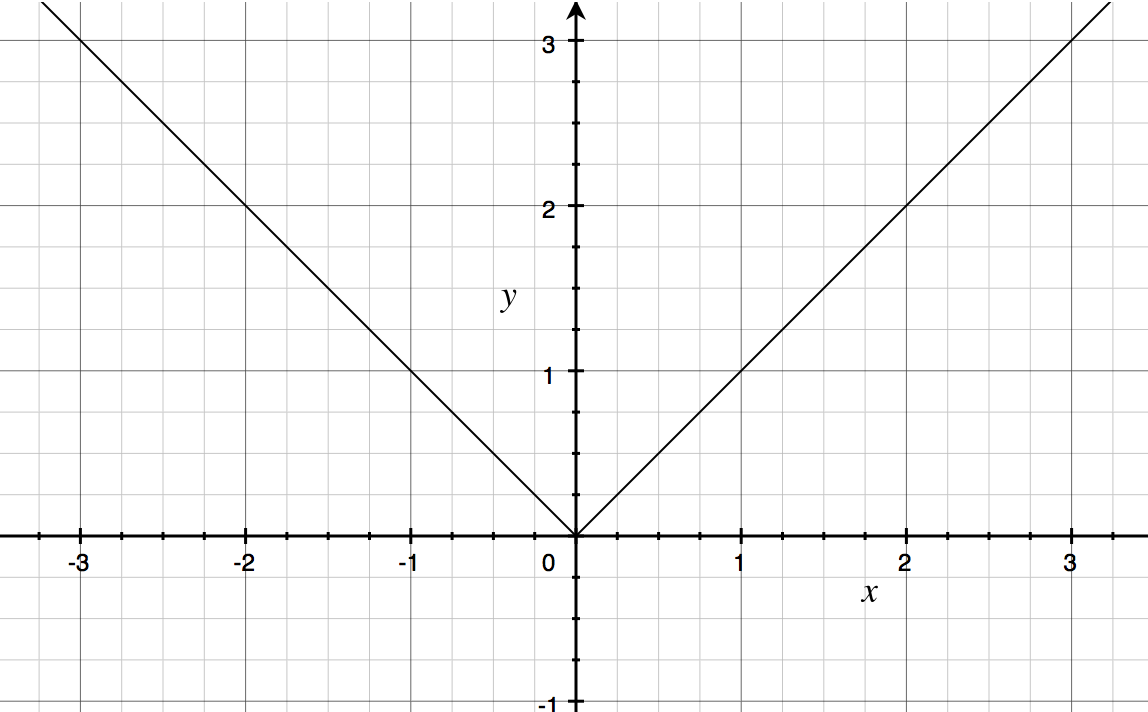
\includegraphics[scale=0.5]{./graphics/absx.png}\\
		$y=|x|$ \emph{is continuous, but not differentiable.}
	\end{center}
	Let $f:D\rightarrow\mathbb{R}$ be a function. Consider the subset
	$$
		C=\{a\in D~|~f'(a)\text{ exists}\}
	$$
	Then one can construct a new function:
	\begin{align*}
		f':C&\rightarrow\mathbb{R}\\
		x&\mapsto f'(x)
	\end{align*}
	If $f(x)=c$, i.e., $f$ is a constant, then
	\begin{align*}
		f'(x)&=\lim_{h\to 0}\frac{f(x+h)-f(x)}{h}\\
		&=\lim_{h\to 0}\frac{c-c}{h}\\
		&=\lim_{h\to 0}\frac{0}{h}=0
	\end{align*}
	Let $n=1,~2,~3,~...$ and consider the function $f(x)=x^n$\\
	Recall the binomial formula:\\
	$$
		(a+b)^n=\left(\begin{array}{c}{n}\\{0}\end{array}\right)a^n+\left(\begin{array}{c}{n}\\{1}\end{array}\right)a^{n-1}b+\left(\begin{array}{c}{n}\\{2}\end{array}\right)a^{n-2}b^2+...+\left(\begin{array}{c}{n}\\{n-1}\end{array}\right)ab^{n-1}+\left(\begin{array}{c}{n}\\{n}\end{array}\right)b^n
	$$
	$$
		=\sum^{n}_{k=0}\left(\begin{array}{c}{n}\\{k}\end{array}\right)a^{n-k}b^k
	$$
	Where $\left(\begin{array}{c}{n}\\{k}\end{array}\right)=\frac{n!}{(n-k)!k!}$
	Then
	\begin{align*}
		f'(x)&=\lim_{h\to 0}\frac{f(x+h)-f(x)}{h}\\
		&=\lim_{h\to 0}\frac{x+h)^n-x^n}{h}\\
		&=\lim_{h\to 0}\frac{ \left[ \sum\limits^n_{k=0}\left(\begin{array}{c}{n}\\{k}\end{array}\right) x^{n-k}h^k \right] -x^n}{h}\\
		&=\lim_{h\to 0}\frac{ \left[ \sum\limits^n_{k=1}\left(\begin{array}{c}{n}\\{k}\end{array}\right) x^{n-k}h^k \right]}{h}\\
		&=\lim_{h\to 0}\left[ \sum\limits^n_{k=1}\left(\begin{array}{c}{n}\\{k}\end{array}\right) x^{n-k}h^{k-1} \right]\\
		&=\left(\begin{array}{c}{n}\\{1}\end{array}\right)x^{n-1}=nx^{n-1}
	\end{align*}
	\pagebreak\\
	\Large{Trigonometry}\\
	\normalsize
	How do your compute the derivative of $y=\sin(x)$?
	\begin{align*}
		\frac{d\sin}{dx}(x)&=\lim_{h\to 0}\frac{\sin(x+h)-\sin(x)}{h}\\
		&=\lim_{h\to 0}\frac{\sin(x)\cos(h)+\sin(h)\cos(x)-\sin(x)}{h}\\
		&=\lim_{h\to 0}\frac{\sin(x)(\cos(h)-1)}{h}+\lim_{h\to 0}\frac{\sin(h)\cos(x)}{h}\\
	\end{align*}
	To help us go beyond those examples, we need "recipes:"\\
	Let $f$ and $g$ two differentiable functions $c\in\mathbb{R}$.
	\begin{itemize}
		\item $(cf)'(x)=cf'(x)$
		\item $(f\pm g)'(x)=f'(x)\pm g'(x)$
		\item $(f\cdot g)'(x)=f'(x)\cdot g(x)+f(x)\cdot g'(x)$
		\item $\left(\frac{f}{g}\right)'(x)=\frac{f'(x)g(x)-f(x)g'(x)}{g(x)^2}$
	\end{itemize}
	Let $f(x)=a^x$ for some $a\in~]0,1[~\cup~]1,+\infty[$
	\begin{align*}
		f'(x)&=\lim_{h\to 0}\frac{a^{x+h}-a^x}{h}\\
		INCOMPLETE
	\end{align*}
	Let's consider two possible $a$, i.e. $a=2$ and $a=3$, and let's approximate in those two cases the limit
	$$
		\lim_{h\to 0}\frac{a^{h}-1}{h}
	$$
	\begin{tabular}{r | c | l}
		\hline
			{1}&{}&{}\\
			{INCOMPLETE}&{}&{}\\
		\hline
	\end{tabular}
	\begin{enumerate}
		\item Tangent line
		\item Velocity
		\item High derivatives
	\end{enumerate}
	\large{Equation of a line}\\
	\normalsize
	Recall that the equation of a line in the plane is $y=mx+b$, where $
\end{document}